% 第一章 绪论
\chapter{绪论}
\section{研究背景}
\subsection{智能驾驶测试对海量长尾场景的需求矛盾}
随着智能驾驶技术的飞速发展,其测试需求也日益复杂和多样化。智能驾驶系统需要在各种复杂多变的交通场景下表现出可靠的性能,以确保驾驶的安全性和舒适性。然而,现实交通环境中存在着海量的长尾场景,这些场景虽然出现频率较低,但一旦发生,往往会对智能驾驶系统构成严峻挑战。
长尾场景的复杂性主要体现在以下几个方面。首先,交通环境的动态性极强,车辆、行人、非机动车等多种交通参与者的行为模式千变万化。例如,在城市道路中,行人可能会突然横穿马路,非机动车可能会随意变道或逆行,这些行为都可能导致潜在的碰撞风险。智能驾驶系统必须能够准确感知和预测这些行为,并做出合理的决策。其次,道路条件的多样性也增加了测试场景的复杂性。从城市快速路到乡村小道,从高速公路到山区道路,不同道路的几何形状、路面状况、交通标志和信号灯等都有所不同。智能驾驶系统需要在这些不同的道路条件下都能正常运行。此外,天气条件和光照条件的变化也会对智能驾驶系统的感知和决策产生影响。雨、雪、雾等恶劣天气会降低传感器的性能,而不同的光照条件(如强光、弱光、逆光等)会影响视觉系统的识别效果。
为了确保智能驾驶系统的安全性和可靠性,测试过程中需要覆盖尽可能多的长尾场景。然而,这面临着巨大的挑战。一方面,长尾场景的数量庞大,几乎无法穷尽。要完全覆盖所有可能的场景几乎是不可能的任务。另一方面,这些场景的出现频率较低,难以在实际道路测试中频繁遇到。因此,传统的测试方法往往难以满足智能驾驶系统对海量长尾场景的测试需求,导致测试的充分性和有效性受到限制。

\subsection{传统场景构建方法的人力成本与效率瓶颈}
在智能驾驶测试领域,传统的场景构建方法主要依赖于人工设计和开发。这些方法虽然在一定程度上能够满足测试需求,但也存在着显著的局限性。
首先,人工设计场景需要大量的专业人员投入。这些人员需要具备深厚的交通工程、计算机科学和智能驾驶技术等多学科知识,能够准确理解和模拟各种复杂的交通场景。然而,这样的人才相对稀缺,培养成本高昂。而且,随着测试需求的不断增加,对专业人员的需求也在持续增长,这进一步加剧了人力成本的压力。
其次,人工设计场景的效率较低。设计一个复杂的交通场景需要经过需求分析、场景建模、代码编写和调试等多个步骤。每个步骤都需要耗费大量的时间和精力。例如,在场景建模阶段,需要精确地定义道路的几何形状、交通参与者的初始位置和行为模式等。在代码编写阶段,需要将这些模型转化为可执行的代码,这不仅需要专业的编程技能,还需要反复调试以确保代码的正确性和稳定性。因此,人工设计场景的速度远远无法满足智能驾驶系统快速迭代和测试的需求。
此外,人工设计场景的准确性和一致性也难以保证。由于不同设计人员的理解和经验不同,可能会导致设计出的场景存在差异。而且,在复杂的场景中,人工设计容易遗漏一些关键的细节,从而影响测试结果的准确性和可靠性。

\subsection{大语言模型在代码生成领域的突破性进展}
近年来,大语言模型(LLM)在自然语言处理领域取得了巨大的突破,并逐渐拓展到代码生成等领域。大语言模型通过在海量文本数据上进行预训练,学习到了语言的语法、语义和逻辑结构,能够生成自然流畅且符合逻辑的文本内容。这种能力为解决智能驾驶测试场景构建的难题提供了新的思路。
在代码生成领域,大语言模型已经展现出了强大的能力。通过对代码数据的学习,大语言模型能够理解代码的结构和逻辑,生成符合语法规范的代码片段。例如,一些基于大语言模型的代码生成工具可以根据用户输入的自然语言描述,自动生成相应的代码实现。这些工具已经在软件开发领域得到了广泛的应用,显著提高了代码开发的效率和质量。
大语言模型在代码生成中的优势主要体现在以下几个方面。首先,它能够快速生成代码,大大缩短了开发周期。传统的人工编写代码需要经过需求分析、设计、编码和调试等多个阶段,每个阶段都需要耗费大量的时间。而大语言模型可以根据输入的描述直接生成代码,减少了中间环节,提高了开发效率。其次,大语言模型生成的代码质量较高。它能够学习到代码的最佳实践和规范,生成的代码不仅符合语法规范,还具有良好的可读性和可维护性。此外,大语言模型还能够根据不同的需求生成多样化的代码实现,为开发者提供了更多的选择。
将大语言模型应用于智能驾驶测试场景构建,可以充分利用其在代码生成领域的优势,解决传统方法面临的困境。通过将自然语言描述的测试场景需求转化为代码实现,大语言模型可以快速生成高保真的测试场景,提高场景构建的效率和质量。同时,结合智能驾驶领域的专业知识,还可以进一步优化大语言模型的性能,使其更好地适应智能驾驶测试场景构建的需求。



	
\section{国内外研究现状}
\subsection{基于大语言模型能够根据人的自然语言指令生成Scenic场景代码}
	随着大语言模型(如GPT-3、T5等)的广泛应用,基于自然语言描述生成仿真场景代码成为自动驾驶仿真研究的一个重要方向。自然语言描述能够以简单、直观的方式传递场景信息,传统的手工编写场景代码的方式效率低且灵活性差,因此,如何利用自然语言生成交通仿真场景脚本成为该领域的核心问题。
	
	大语言模型的应用:大语言模型,如GPT-3和T5,已经被成功应用于自然语言到场景代码的转换。通过训练,这些模型能够理解复杂的自然语言输入,并根据描述生成结构化的Scenic脚本。这些模型通过解析用户的自然语言指令,生成符合自动驾驶仿真要求的场景代码。例如,\textbf{Chen et al. (2022)}提出了一种基于GPT的框架,能够根据自然语言描述生成完整的交通场景配置,包括车辆、行人、交通灯等元素。
	
	挑战与进展:尽管大语言模型在生成场景代码上取得了一定的进展,仍然面临一些挑战。首先,如何处理自然语言中的歧义和模糊性是一个难题,特别是在复杂场景描述下,生成的场景可能无法完全符合预期。其次,现有模型的生成能力在处理非常复杂或特殊的交通场景时可能存在局限性。因此,如何增强语言模型的语义理解和场景生成的准确性,仍然是一个活跃的研究领域。
	
	\subsection{将场景代码合成合理的智能驾驶场景}
	将生成的Scenic场景代码转化为合理的智能驾驶仿真场景,是实现自动驾驶测试和验证的关键步骤。生成的场景不仅需要符合交通规则,还要能够模拟真实的驾驶环境,以便进行有效的测试。
	
	场景代码到仿真环境的转化:目前的研究主要集中在如何将由大语言模型生成的Scenic脚本转化为仿真平台可执行的场景配置。例如,\textbf{Xie et al. (2021)}开发了基于Scenic的编译器,能够将自然语言生成的场景描述转化为CARLA仿真平台所需的配置文件。通过这种方式,生成的场景能够在高保真的仿真环境中进行验证。
	
	智能场景合成与动态行为建模:智能驾驶场景不仅包括静态元素(如道路、交通标志等),还包括动态行为(如车辆行驶、变道、停车等)。研究者们提出了多种动态行为建模方法,使得生成的交通场景能够更真实地反映驾驶行为和交通流。例如,\textbf{Zhao et al. (2020)}提出了一种基于行为模型的动态场景合成方法,通过模拟交通参与者的行为,生成交互式的智能驾驶环境。
	
	复杂交通场景的挑战:尽管场景合成方法不断发展,如何生成复杂、真实且符合交通规则的场景仍然是一个技术挑战。现有的场景生成方法在处理复杂交通场景时,可能出现车辆行为不自然、交通规则不严谨等问题。因此,如何提高场景合成的灵活性和复杂性,仍然是研究的重点。
	
	\subsection{对生成的交通场景进行展示和效果的量化衡量}
	生成交通场景后,对其进行展示和量化评估是确保场景质量和仿真结果准确性的关键。通过对场景的可视化和量化评估,研究人员能够验证场景的有效性,并为后续的自动驾驶算法优化提供数据支持。
	
	可视化展示:生成的交通场景可以通过可视化工具展示,以便人工验证和审阅。\textbf{Dai et al. (2020)}提出了一种基于关键帧截取的可视化方法,通过仿真过程中截取关键帧图像,帮助研究人员快速了解仿真过程中的交通场景。结合深度学习技术,自动驾驶系统还能够从这些图像中提取重要信息,进行场景的进一步分析和优化。
	
	量化评估指标的提出:为了系统地评估生成场景的质量,许多研究提出了量化评估框架。例如,\textbf{Dai et al. (2020)}提出了一种多维度的评估方法,涵盖了场景的语义保真度、交通密度、车辆行为等多个方面。这些评估指标不仅能够反映生成场景的真实性,还能够帮助研究人员评估仿真结果的有效性。
	
	安全性与性能评估:自动驾驶系统在仿真环境中的表现也需要量化评估。\textbf{Li et al. (2021)}提出了一种基于自动驾驶系统安全性的评估框架,通过分析车辆在生成场景中的碰撞率、通过率等指标,评估自动驾驶系统在不同场景下的安全性和稳定性。通过这样的量化评估,研究人员能够识别潜在的风险和问题,进一步优化自动驾驶算法。
	
	\section{研究内容}
	\subsection{面向场景描述的领域知识图谱构建}
	在自动驾驶测试场景生成中,构建面向场景描述的领域知识图谱是实现高效、准确场景生成的基础。领域知识图谱通过整合自动驾驶领域的专业知识,包括交通规则、道路类型、车辆行为模式、传感器特性等,为自然语言描述的解析和形式化代码的生成提供丰富的上下文信息和语义支持。
	
	领域知识图谱的构建涉及多个关键步骤。首先,需要对自动驾驶领域的知识进行系统梳理和分类,明确知识的层次结构和关联关系。这包括对交通场景中的实体(如车辆、行人、道路、交通标志等)及其属性(如位置、速度、类型等)的定义,以及这些实体之间的关系(如车辆与道路的交互、车辆与行人的避让等)。通过构建知识图谱,可以将这些复杂的知识结构化地表示出来,便于后续的查询和推理。
	
	在知识图谱的构建过程中,还需要考虑知识的动态更新和扩展。自动驾驶技术不断发展,新的交通规则、车辆类型和传感器技术等不断涌现,因此知识图谱需要具备良好的可扩展性和可更新性。通过持续的知识更新,可以确保知识图谱始终保持最新状态,从而为场景生成提供准确的知识支持。
	
	此外,领域知识图谱的构建还需要考虑知识的表达和存储方式。知识图谱通常以图的形式存储,其中节点表示实体,边表示实体之间的关系。这种结构化的存储方式不仅便于知识的查询和推理,还能够支持复杂的知识融合和关联分析。通过知识图谱的构建,可以实现对自动驾驶场景描述的深度理解和语义解析,为后续的代码生成和场景合成提供坚实的基础。
	
	\subsection{基于LLM的语义约束代码生成方法}
	基于大型语言模型(LLM)的语义约束代码生成方法是实现自动驾驶测试场景高效生成的关键技术之一。LLM具有强大的语言理解和生成能力,能够根据自然语言描述生成高质量的形式化代码。然而,为了确保生成代码的准确性和可靠性,需要在代码生成过程中引入语义约束机制。
	
	语义约束代码生成方法的核心在于将自然语言描述的语义信息转化为代码生成的约束条件。这些约束条件可以包括交通规则、道路类型、车辆行为模式等,确保生成的代码不仅符合语法规范,还满足实际场景的语义要求。通过语义约束机制,可以有效避免生成代码中的逻辑错误和不符合实际场景的情况,提高代码的质量和可用性。
	
	在实现语义约束代码生成时,需要充分利用LLM的语言理解和生成能力。LLM可以通过对自然语言描述的深度理解,提取出关键的语义信息,并将其转化为代码生成的约束条件。同时,还需要开发相应的算法和工具,将这些约束条件嵌入到代码生成过程中,确保生成的代码能够准确地反映自然语言描述的语义内容。
	
	此外,语义约束代码生成方法还需要考虑代码的可读性和可维护性。生成的代码不仅需要符合语法和语义规范,还需要具有良好的结构和注释,便于后续的修改和扩展。通过基于LLM的语义约束代码生成方法,可以实现从自然语言描述到形式化代码的高效转换,为自动驾驶测试场景的生成提供强大的技术支持。
	
	\subsection{场景物理合理性的多模态验证机制}
	场景物理合理性的验证是自动驾驶测试场景生成中的一个重要环节,它直接影响到测试场景的真实性和可靠性。为了确保生成场景的物理合理性,需要建立一种多模态验证机制,通过多种方式对场景进行综合验证。
	
	多模态验证机制的核心在于结合多种验证手段,从不同角度对场景的物理合理性进行评估。这些验证手段可以包括基于物理规则的验证、基于仿真数据的验证以及基于专家知识的验证等。通过多种验证手段的结合,可以全面评估场景的物理合理性,确保生成的场景符合实际交通环境的物理规律。
	
	基于物理规则的验证是多模态验证机制的重要组成部分。通过定义和应用物理规则,如牛顿运动定律、能量守恒定律等,可以对场景中的物体运动和交互进行验证。例如,可以验证车辆的加速度是否符合物理规律,车辆与行人之间的碰撞是否符合能量守恒等。

\section{本文研究框架}

为实现基于自然语言输入自动生成高保真三维交通场景并进行量化评估的目标,本文构建了一个集自然语言处理、交通场景建模、三维仿真与量化评估于一体的综合研究体系。整体研究框架如下:

首先,本文分析当前国内外在自然语言驱动的场景生成、智能仿真系统集成与自动驾驶场景评估方面的研究进展,明确研究问题与技术挑战。

随后,围绕\textbf{“自然语言 → 场景代码 → 三维仿真 → 评估指标”}这一主线,设计并实现一个端到端自动化系统,涵盖以下三个关键研究方向:

\begin{enumerate}
	\item \textbf{基于大语言模型的Scenic场景代码生成技术} \\
	研究如何借助预训练大语言模型(如GPT-4o)结合检索增强机制(如Sentence-T5)解析自然语言指令,生成符合语义的交通场景描述脚本(Scenic)。重点解决生成脚本的语义准确性与交通合理性问题。
	
	\item \textbf{交通场景代码到三维仿真的合成机制} \\
	研究如何将自然语言生成的场景脚本有效地转换为可运行的三维智能驾驶仿真场景。通过Scenic语言与CARLA仿真平台的集成,实现车辆、行人、环境等交通要素在虚拟世界中的构建与动态演化。
	
	\item \textbf{生成场景的展示与量化评估方法} \\
	建立多维度评估体系,从语义保真度、多样性和驾驶性能三个方面量化分析生成场景的质量与有效性。设计自动化指标计算方法,并结合视觉展示手段增强实验可解释性。
\end{enumerate}

在上述研究基础上,本文完成了系统的整体实现与实验验证,验证了所提出方法的有效性,并总结了本研究的创新点与潜在改进空间。

\begin{figure}[H]
	\centering
	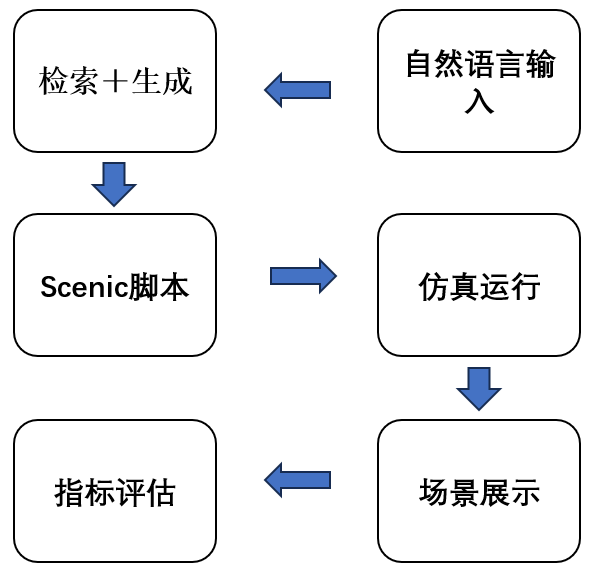
\includegraphics[width=0.9\textwidth]{../images/研究架构图.png} 
	\caption{本文的研究框架}
	\label{fig:research_framework}
\end{figure}
